\documentclass[12pt]{article}
\usepackage[english]{babel}
\usepackage[utf8x]{inputenc}
\usepackage[T1]{fontenc}
\usepackage{scribe}
\usepackage{listings}
\usepackage{float}
\usepackage{amsmath}

\Scribe{Group 9,10}
\Lecturer{Prof. Abir De}
\LectureNumber{5}
\LectureDate{January 27, 2023}
\LectureTitle{Understanding Generalization and Overfitting}

\lstset{style=mystyle}

\begin{document}
\MakeScribeTop


\section{Introduction}

Generalization refers to your model's ability to adapt properly to new, previously unseen data, drawn from the same distribution as the one used to create the model. It is the ability of a model to undergo training and validation, followed by its  ability to match the values i.e performance on the unseen dataset. In this lecture we go across various topics involving errors, model complexity,  concepts such as variance, bias and noise following it up with Bias-Variance Analysis in Regression.

\section{Error and Model Complexity}

In machine learning, model complexity and overfitting are related in a manner that model overfitting is a problem that can occur when a model is too complex due to different reasons. This can cause the model to fit the noise in the data rather than the underlying pattern. As a result, the model will perform poorly when applied to new and unseen data. 

\subsection{What is Model Complexity?}

Model complexity is a key consideration in machine learning. Simply put, it refers to the number of predictors or independent variables or features that a model needs to take into account in order to make accurate predictions. In our case we are taking a polynomial model to help better understand the subject matter.

\subsection{Polynomial Case Analysis to discuss Underfitting vs Overfitting}

Suppose we consider $N$ training data points. We take a polynomial of degree $d$, and the number of parameters is $d+1$. Here we discuss the complexity in terms of number of parameters. More the value of $d$, more is the degree of the polynomial, more fitting is generated. Lesser the value of $d$, lesser is the degree of polynomial and fitting, but more errors on the training set.

\begin{figure}[H]
    \centering
    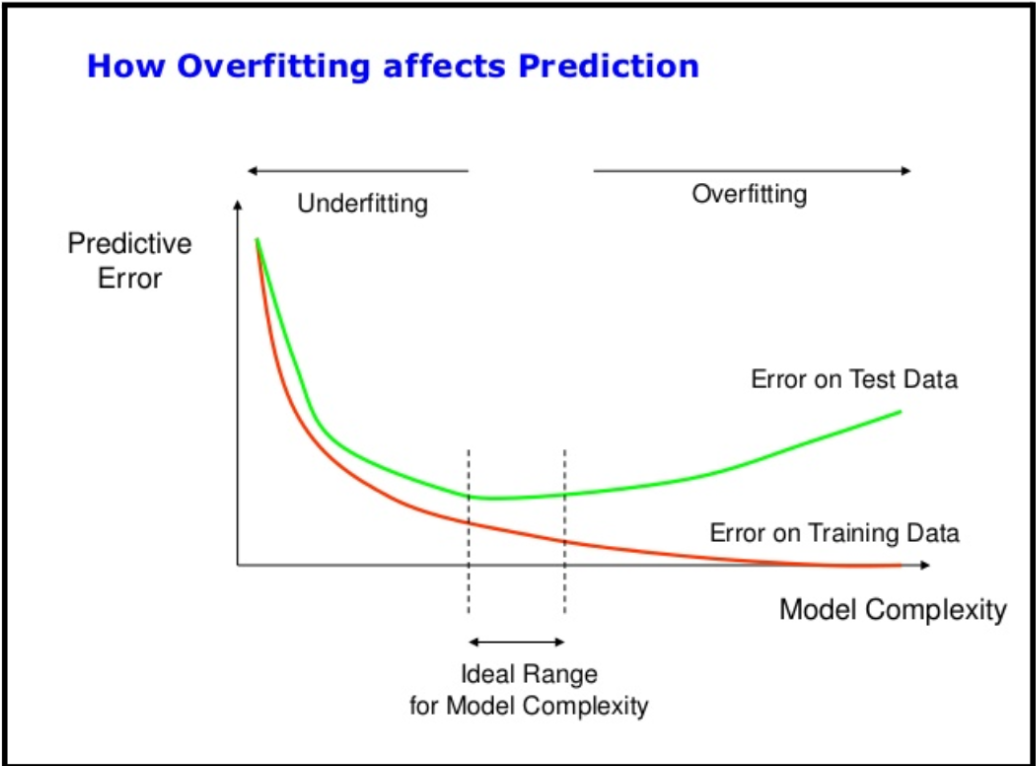
\includegraphics[width=\linewidth]{Model Complexity v_s Errors.png}
    \caption{Plot of Model Complexity v/s Errors}
    \label{fig:mcvse}
\end{figure} 

\noindent
\textbf{Discussion of the Plot:}\newline
Referring to plot in figure - \ref{fig:mcvse}, we start increasing the value of $d$ from $0.1$ to a higher value. So we move from a linear function to a higher degree of polynomial. As we can see, we see a high value of error both on the training and the test dataset at very low values of $d$. As the value of $d$ increases, the error starts to decrease until a point where the error on the test data undergoes a minima. 
\\ By common sense, the error in the training data set is a strictly decreasing function of d, as overfitting continues to happen. After the minima on the error in the test set, the error starts to increase on increasing value of d. The reason behind it being that we start to account for even the noises in the data causing overfitting leading to deviation from the original value of the underlying function. Some other things to note that were discussed in class:
\begin{itemize}
    \item The value of error on training data decreases rapidly initially after which the slope of the decline reduces, suggesting that no drastic change in error in increasing order of polynomial from $d$ to $d+1$ at high values of $d$. Coefficient of $x^{(d+1)}$ term is small
    \item In general, value of validation error (error on test data) is more than error on training data
\end{itemize}

\subsection{Overfitting}
\noindent Overfitting is when the model we have trained fits the training dataset too well, such that it fails to be general enough for the validation or test set. This can happen in the following cases:
\begin{itemize}
    \item The training data is too small
    \item The model is too complex
    \item The data used for training is not cleaned and contains garbage values. The model captures the noise in the training data and fails to generalize the model's learning
\end{itemize}

\noindent In a sense, the model learns "too much" from the dataset.\\

\begin{figure}[H]
    \centering
    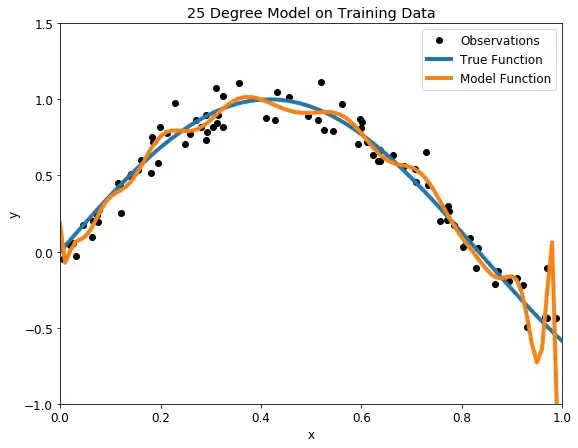
\includegraphics[width=.5\textwidth]{Overfit.jpg}
    \caption{Example of Overfitting}
    \label{Figure 2}
\end{figure}

\noindent An example would be trying to fit a simple linear dataset having some noise using a very high degree polynomial. This leads to very low training error but high validation error and is thus undesirable.\\

\subsection{Underfitting}
\noindent Underfitting is when the model we have trained is too simple for the dataset it is being trained upon. An example would be trying to fit an exponential curve with a linear classifier. It can happen in the following cases:
\begin{itemize}
    \item The model is assumed to be too simple
    \item The dataset is too complex for the model
    \item Unclean training data containing noise or outliers can be a reason for the model to not be able to derive patterns from the dataset
\end{itemize}

\noindent So, we are trying to learn a very complex dataset with very few parameters. Thus we have high training as well as high validation error in this case. This is also undesirable.\\

\begin{figure}[H]
    \centering
    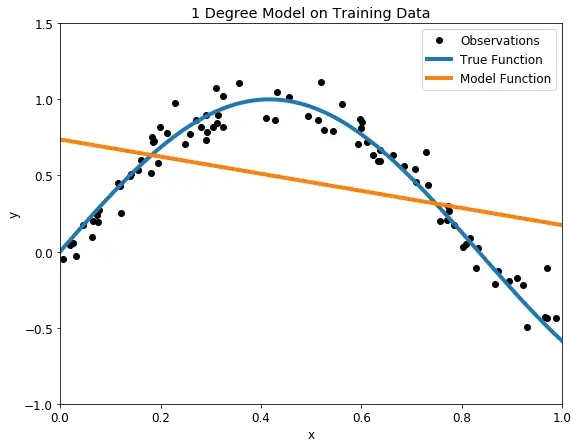
\includegraphics[width=.5\textwidth]{Underfit.jpg}
    \caption{Example of Underfitting}
    \label{Figure 3}
\end{figure}

\subsection{How to solve overfitting and underfitting?}
We are just mentioning the solutions and won't be going over them in detail in this lecture.\\

\noindent \textbf{For overfitting:}
\begin{itemize}
    \item Train with more data
    \item Data augmentation
    \item Feature selection (removing redundant features)
    \item Cross-validation (like K-fold cross-validation or bootstrap sampling)
    \item Reduce complexity of model
    \item Regularization
    \item Ensembling
    \item Early Stopping
    \item Adding dropouts (for large Neural Networks)
\end{itemize}

\noindent \textbf{For underfitting:}
\begin{itemize}
    \item Decrease regularization
    \item Increase the duration of training
    \item Introducing more features
    \item Removing noise from the data
\end{itemize}

\subsection{Conclusion: Striking a Balance between both}
Hence the conclusion drawn is: A model with a high degree of complexity ( higher $d$ value) may be able to capture more variations in the data, but it will also be more difficult to train and may be more prone to overfitting. On the other hand, a model with a low degree of complexity (lower $d$ value) may be easier to train but may not be able to capture all the relevant information in the data. Thus, we have a trade-off between overfitting and underfitting and the best fit is in between these. This is also referred to as Bias-Variance tradeoff. Finding the right balance between model complexity and predictive power is crucial for successful machine learning. 


\section{Main Sources of Test Error}
In machine learning, there are three main causes of errors that we need to analyze in order to improve our algorithm and optimize our model. These main sources of error are:
\begin{enumerate}
    \item Bias
    \item Variance
    \item Noise
\end{enumerate}
We’ll discuss each of them in detail in the coming few paragraphs.

\subsection{Bias}
Bias is the difference between the average prediction of our model and the correct value which we are trying to predict. In simple terms it can also be stated as the difference between the truth and the best prediction function we have in our modeling space.\\ 
Bias is a systematic error in a sense that it happens in the model due to incorrect assumptions while training the model. Models with high bias are rigid and oversimplify the issue, resulting in high training errors and poor performance on unseen data.
\subsection{Variance}
Variance is a measure of the fluctuations between the learned functions across different training datasets. In simple terms, variance measures the variability of the model to the dataset i.e. how well does the model change depending on the dataset. Models with high variance are sensitive to small changes in data and fit the training set too closely, leading to low training error but high test error.
\subsection{Noise}
Noise is a random error in input data that can impact a machine learning model's predictions. It may originate from sources such as measurement errors, incorrect labels, or outliers. Noise makes it difficult for the model to accurately capture the relationship between inputs and outputs, leading to unpredictable and inconsistent predictions.
\subsection{Conclusion}
Achieving good performance on both training and test data requires striking a balance between bias and variance in machine learning models. This can be done through selecting an appropriate model complexity, using regularization techniques, and incorporating cross-validation.


\section{Bias Variance Analysis in Regression}
Bias-variance analysis is used to evaluate the performance of a machine learning model. The main idea is to decompose the total prediction error into three sources of error: bias, variance and noise. \\ Let's suppose our true function is of the following form
\begin{align}
    y = g(x)+\epsilon
\end{align}
where $E$ is the error function with $\mu=0$ and variance $\sigma^2$. Our prediction model can be expressed as follows
\begin{align}
    f_D(x) = \omega^Tx
\end{align}
Bias can be formulated as follows\\ 
\begin{align}
\begin{split}\label{eq:1}
    Bias ={}& \left(E_{D}[f_D(x)]-g(x)\right)^2 \\
    ={}& (E_{D}[f_D(x)])^2 - 2E_{D}[f_D(x)]g(x) + g(x)^2
\end{split}
\end{align}
Variance can be formulated as follows
\begin{align}
\begin{split}\label{eq:2}
    Variance ={}& E_{D}[(f_D(x)-E_D[f_D(x)])^2]\\
    ={}& E_D[(f_D(x))^2]-E_D[f_D(x)]^2
\end{split}
\end{align}
Noise can be formulated as follows
\begin{align}
\begin{split}\label{eq:3}
    Noise ={}& E_{\epsilon}[(y-g(x))^2] \\
    ={}& E_{\epsilon}[y^2 - 2yg(x) + (g(x))^2] \\
    ={}& E_{\epsilon}[y^2] - E_{\epsilon}[2yg(x)] + (g(x))^2 \\
    ={}& E_{\epsilon}[y^2] - 2E_{\epsilon}[(g(x))^2 + \epsilon g(x)] + (g(x))^2 \\
    ={}& E_{\epsilon}[y^2] - 2(g(x))^2 + (g(x))^2
\end{split}
\end{align}
We can already see that some of the terms cancel out, we can write the sum of the above three errors as follows
\begin{align}
\begin{split}\label{eq:4}
    Bias + Variance + Noise ={}& E_{\epsilon}[y^2] - 2E_{D}[f_D(x)]g(x) + E_{D}[(f_D(x))^2]
\end{split}
\end{align}
Now we write the total prediction error and show that it equals the total sum of above bias, variance and noise.
\begin{align}
\begin{split}\label{eq:5}
    E_{D,\epsilon}[(y-f_D(x))^2] ={}& E_{D,\epsilon}[y^2] - E_{D,\epsilon}[2yf_D(x)] + E_{D,\epsilon}[(f_D(x))^2] \\
    ={}& E_{\epsilon}[y^2] - 2E_{D}[g(x)f_D(x)] - 2E_{\epsilon}[\epsilon f_D(x)]+ E_{D}[(f_D(x))^2] \\
    ={}& E_{\epsilon}[y^2] - 2E_{D}[f_D(x)]g(x) + E_{D}[(f_D(x))^2] \\
    ={}& Bias + Variance + Noise
\end{split}
\end{align}
Hence proved that the total prediction error equals the total sum of bias, variance and noise. \\ Post this proof, sir emphasized on the fact that even if our model is optimal in terms of minimizing the Bias and Variance losses, we can never get an expected total prediction error that is less than the noise error. \\

\end{document}
